% This paper follows the LLNCS macro package for Springer Computer Science
% proceedings; based on samplepaper.tex, Version 2.21 of 2022/01/12.
%
% English edition of reports/lncs_phuong_phap.tex. The Vietnamese file is kept
% as-is; the two are meant to stay in step, so a change to one belongs in the
% other as well.
%
\documentclass[runningheads]{llncs}
%
% ---------------------------------------------------------------------
% FONT ENCODING
% The body of this paper is English, for which the sample's [T1] would be
% correct. We keep [T5] for one reason only: the author names carry Vietnamese
% diacritics that T1 cannot render. T5 covers the full ASCII range, so English
% text sets exactly as it would under T1.
% ---------------------------------------------------------------------
\usepackage[utf8]{inputenc}
\usepackage[T5]{fontenc}
%
\usepackage{graphicx}
\usepackage{amsmath}
\usepackage{amssymb}
% The pipeline figure is drawn in TikZ, i.e. vector graphics, as the sample
% recommends for diagrams and schematics.
\usepackage{tikz}
\usetikzlibrary{arrows.meta, positioning}
%
\begin{document}
%
% No \renewcommand block here: llncs already labels everything in English.
%
\title{Two-Stage Fusion for Routing and Classification in
Parameter-Efficient Continual Learning}
%
\titlerunning{Two-Stage Fusion for PET-Based Continual Learning}
%
% ORCID iDs not yet available; \orcidID{} omitted for now. Fill in before
% the final submission.
\author{Nguyễn Thiên Trường \and Tống Quang Thái}
%
\authorrunning{N. T. Trường and T. Q. Thái}
%
\institute{University of Engineering and Technology,\\
Vietnam National University, Hanoi, Vietnam\\
\email{24022480@vnu.edu.vn, 24022450@vnu.edu.vn}}
%
\maketitle
%
\begin{abstract}
Continual learning methods built on parameter-efficient tuning maintain a
lightweight parameter pool, one set per task, and at inference must decide which
set to attach to the backbone before classifying. That decision is made from a
single source of evidence, so everything downstream is capped by the quality of
one module. We show that a second source of evidence is already present inside
the trained model and can be read out without any gradient training: a
second-order classification head built on a frozen random projection of the
existing LoRA features, whose weights are the closed-form ridge solution of
statistics accumulated one task at a time. This source is fused at two points,
both at inference time. The first stage blends it with the original routing
signal after standardising the two sources onto a common scale. The second stage
uses it as a secondary classifier, weighted per sample in inverse proportion to
how decided the primary classifier already is, so that the blend opens only on
contested samples. Across three continual-learning benchmarks and four seeds,
routing accuracy rises by $+1.10$ to $+2.26$ points and classification accuracy
by $+0.69$ to $+1.50$ points; on both axes the gain is several times the
seed-to-seed standard deviation. The two retention metrics show no change
distinguishable from zero. The head costs one extra forward pass per sample and
a closed-form solve per task.

\keywords{Continual learning \and Parameter-efficient tuning \and Parameter
routing \and Random projection \and Signal fusion.}
\end{abstract}
%
%
%
\section{Introduction}

A continual learner built on parameter-efficient tuning keeps one lightweight
parameter set per task and, at inference, must decide which set to attach to the
frozen backbone before it can classify. That decision is made once, from a
single module, and everything downstream inherits it: a wrong choice attaches
the wrong adapter, and the classifier that follows is asked to work from
features it was not adapted for. Successive methods in this line have improved
the decision --- richer pools, attention-weighted combinations, explicit
re-matching stages --- but none change the fact that one signal stands in front
of the rest of the pipeline.

We observe that a second, independent source of evidence is already present
inside such a trained model and is simply discarded. The LoRA features that the
pipeline computes anyway can be pushed through a fixed random projection and
read by a closed-form ridge classifier built from second-order statistics. Its
output weights are fitted --- solving a supervised least-squares problem is
learning, whatever the solver --- but they are obtained in closed form rather
than by gradient descent, from running sums rather than from stored examples,
and without touching the backbone, the adapters or the training loop. The head
retains no images and no per-sample features, and adds one adapter forward per
sample at inference. More importantly it fails on \emph{different samples}
than the routing module does, which is the property that makes combining them
worthwhile rather than redundant.

The paper puts that second source to work at the two points where the original
pipeline commits to a decision. At the routing level it is blended with the
existing task signal after both are standardised onto a common scale. At the
classification level it is used as what it already is --- a complete classifier
--- weighted per sample so that the blend opens only where the primary
classifier is undecided.

\subsubsection{Contributions.}
\begin{itemize}
\item We identify two weaknesses in the re-matching pipeline of
      HRM-PET~\cite{ref_hrmpet}: its routing signal comes from one module, and a
      better route does not automatically become a better prediction because the
      shared head frequently predicts the correct class in spite of a wrong
      route (Sect.~\ref{sec:method}).
\item We show that a training-free second-order head over a frozen random
      projection of the existing features supplies a second source of evidence
      whose errors are decorrelated from the first, and we fuse the two at both
      the routing and the classification level, entirely at inference time.
\item We evaluate on three datasets over four seeds and report by axis: routing
      improves by $+1.10$ to $+2.26$ points and classification by $+0.69$ to
      $+1.50$, each several times the seed-to-seed standard deviation, while the
      two retention metrics show no change we can resolve and we claim none
      (Sect.~\ref{sec:results}).
\item We reconstruct the full grid the original work covers --- four datasets by
      five pre-training configurations, identified from traces in its released
      code. All $20$ cells improve on both accuracy axes, over baselines that
      span from $31.8$ to $93.8$ Acc@1 (Sect.~\ref{sec:grid}).
\end{itemize}

\subsection{Problem Statement}

Class-incremental learning (CIL) learns a sequence of $T$ tasks without
forgetting earlier ones. The $t$-th task consists of $n_t$ samples
$\mathcal{D}_t=\{(x^t_i,y^t_i)\}_{i=1}^{n_t}$ drawn from a class set
$\mathcal{C}_t$, where $x^t_i \in \mathcal{X}$ is an input image and
$y^t_i \in \mathcal{Y}$ its label.

Three constraints define the setting. At step $t$ only $\mathcal{D}_t$ is
available for training. The class sets are disjoint,
$\mathcal{C}_t \cap \mathcal{C}_{t'} = \emptyset$ for all $t \neq t'$, and at
inference the \emph{task identity is unknown}: the model must discriminate among
all classes seen so far through a single shared classification head. Finally,
this work operates in the exemplar-free setting: images from past tasks are
never retained.

In methods based on parameter-efficient tuning
(PET)~\cite{ref_l2p,ref_dualprompt,ref_hide}, a pre-trained backbone
$h_{\mathrm{ptm}}$ with parameters $\theta_{\mathrm{ptm}}$ is frozen and a
lightweight parameter pool $\mathcal{P}=\{p_1,\dots,p_T\}$ is maintained, each
set trained on one task; here every $p_t$ is a LoRA adapter~\cite{ref_lora}. The
shared classification head is denoted $g_{\theta_g}$. Because the task identity
is unknown at inference, the system is forced to \emph{choose} which parameter
set to attach to the backbone before classifying, and everything downstream
depends on that choice. Table~\ref{tab:notation} summarises the notation used
throughout.

\begin{table}
\small
\setlength{\tabcolsep}{4.5pt}
\caption{Notation used in this paper.}\label{tab:notation}
\begin{tabular}{ll}
\hline
Symbol & Meaning\\
\hline
$\mathcal{D}_t$, $\mathcal{C}_t$ & data and class set of task $t$\\
$h_{\mathrm{ptm}}$, $\theta_{\mathrm{ptm}}$ & pre-trained backbone, frozen\\
$\mathcal{P}=\{p_1,\dots,p_T\}$ & LoRA parameter pool, one set per task\\
$g_{\theta_g}$, $g_\omega$ & shared classification head; auxiliary classifier of TII\\
$q(x)$ & query feature from the bare backbone\\
$\hat{d}(x)$, $\tilde{d}(x)$ & class distribution of TII; of the routed classifier\\
$\mathcal{T}(\cdot)$ & map from class to task identity\\
$\hat{t}_f$, $\hat{t}_s$ & task identity at first matching and after re-matching\\
$u \in \mathbb{R}^{|\mathcal{Y}|}$ & class scores of TII's auxiliary classifier; input to stage 1\\
$\ell \in \mathbb{R}^{|\mathcal{Y}|}$ & class scores of the routed classifier; input to stage 2\\
$s \in \mathbb{R}^{|\mathcal{Y}|}$ & class scores of the random-projection head\\
$z(\cdot)$ & per-sample standardisation, population std floored at $10^{-6}$\\
\hline
\end{tabular}
\end{table}

\subsection{The HRM-PET Baseline Pipeline}

We take HRM-PET~\cite{ref_hrmpet} as our baseline. Its inference pipeline
consists of four modules in sequence, presented in the order the data passes
through them.

\subsubsection{Task-identity inference (TII).}
The input image is passed through the \emph{bare} backbone, with no adapter
attached, to obtain a query feature. That feature enters an auxiliary classifier
$g_\omega$ trained with cross-entropy, producing a distribution over classes:
\begin{equation}
q(x) = h(x;\theta_{\mathrm{ptm}}),
\qquad
\hat{d}(x) = g\!\left(q(x); \theta_\omega\right).
\label{eq:tii}
\end{equation}
The initial task identity is the task containing the highest-probability class,
with $\mathcal{T}$ the class-to-task map.

\subsubsection{Direct and confidence-based re-matching (DRM, CRM).}
Two modules then try to repair a wrong initial match, neither of them trained.
DRM attaches $p_{\hat{t}_f}$, reads the shared head's prediction, and takes the
task of that prediction, $\hat{t}_s$, whenever it disagrees with $\hat{t}_f$;
knowledge shared across the pool means the predicted class often already belongs
to the right task even when the initial match was wrong. Because the substitute
is used only on disagreement, the worst case is a wrong prediction $\hat{t}_f$
would have produced anyway, so the step cannot degrade accuracy.

When the two agree DRM has nothing to substitute, and CRM takes over. Each
parameter set was trained only alongside the classes of its own task, so a
mismatched sample yields a less decided predictive distribution. CRM scores the
$N=2$ highest-probability classes of $\hat{d}(x)$ by a generalised posterior
entropy of the head's output under each candidate's adapter --- no extra
training needed --- and keeps the most confident. Each candidate costs one
further forward pass, which is why $N$ is kept small.

\subsubsection{Shared classification head.}
The selected parameter set is attached to the backbone, and the shared head
produces a score vector over all classes seen so far:
\begin{equation}
\ell = g\!\left(h(x; p_{\hat{t}}, \theta_{\mathrm{ptm}}); \theta_g\right)
   \in \mathbb{R}^{|\mathcal{Y}|},
\qquad
\hat{y} = \arg\max_c\, \ell_c ,
\label{eq:logits}
\end{equation}
where $\hat{t}$ is the identity after DRM and CRM. Classes not yet seen are
masked with $-\infty$.

\subsubsection{First weakness: one routing signal.}
The whole four-module chain depends on \emph{one} routing signal, produced at
(\ref{eq:tii}); DRM and CRM refine it and add no further source. To see what a
second source would be worth we built the random-projection head of
Sect.~\ref{sec:method} on HRM-PET's own LoRA features and used it as a router.
Table~\ref{tab:routing} measures both, and the last row measures their union ---
the fraction of samples at least one of them routes correctly, that is the
ceiling any combination of the two could reach.

\begin{table}
\small
\setlength{\tabcolsep}{4.5pt}
\caption{Routing accuracy (\%), seed 42. The last row is the fraction of samples
at least one of the two routers gets right, i.e.\ the ceiling available to a
combination of the two.}\label{tab:routing}
\begin{tabular}{lrrr}
\hline
Routing source & ImageNet-R & CIFAR-100 & CUB-200\\
\hline
TII                       & 63.80 & 81.21 & 92.96\\
HRM-PET after DRM and CRM & 77.79 & 89.82 & 93.21\\
RP head                   & 77.12 & 89.51 & 94.02\\
\hline
Union of TII and RP head  & \textbf{82.99} & \textbf{92.86} & \textbf{96.26}\\
\hline
\end{tabular}
\end{table}

The two routers fail on \emph{different} samples. On ImageNet-R the union
exceeds TII by $19.19$ points of the whole test set, and since TII is wrong on
$36.20\%$ of it, those points are $53.0\%$ of TII's errors repaired by the
projection head; the same figures are $62.0\%$ on CIFAR-100 and $46.9\%$ on
CUB-200. That complementarity is the necessary condition for fusion to mean
anything --- had the two failed on the same samples, their union could not
exceed the stronger of them, and it exceeds both by more than five points. The
union is an oracle: it uses the labels to ask what a perfect combiner could
reach, and no router we build attains it.

\subsubsection{Second weakness: better routing is not better classification.}
$\ell$ in (\ref{eq:logits}) comes from the \emph{shared} head, which spans every
class seen so far, so a mis-routed sample is frequently classified correctly
anyway. Correcting its route then buys nothing, and re-routing a sample that was
already correct can break it. Empirically the routing gain converts into
classification accuracy at only $14$--$21\%$, and on CUB-200 not at all.

The RP head, however, is not merely a router: it is a complete classifier that
the routing stage discards. Table~\ref{tab:cls} measures the complementarity at
that level.

\begin{table}
\small
\setlength{\tabcolsep}{4.5pt}
\caption{Complementarity at the classification level (\%), seed 42. The last
column is the fraction of samples the routed head gets wrong and the RP head
gets right.}\label{tab:cls}
\begin{tabular}{lrrrr}
\hline
Dataset & Routed head & RP head & Union & RP-only correct\\
\hline
ImageNet-R & 74.31 & 70.08 & 78.89 & $+4.58$\\
CIFAR-100  & 89.97 & 88.76 & 92.40 & $+2.43$\\
CUB-200    & 86.48 & 87.50 & 90.35 & $+3.87$\\
\hline
\end{tabular}
\end{table}

Even on ImageNet-R, where the RP head is four points weaker overall, it
classifies correctly $4.58\%$ of the samples the primary head cannot handle.
These two measurements lead directly to the two components proposed in
Sect.~\ref{sec:method}: the first fuses at the routing level, the second uses
the same head as a second classifier.

\section{Related Work}
\label{sec:related}

\subsubsection{Parameter pools and the selection they require.}
L2P~\cite{ref_l2p} and DualPrompt~\cite{ref_dualprompt} set the shape most
parameter-efficient continual learners still follow: freeze the backbone, keep a
pool of lightweight parameter sets, and pick from it at inference using a query
from the bare backbone. CODA-Prompt~\cite{ref_coda} replaces the discrete pick
with an attention-weighted combination; HiDe-Prompt~\cite{ref_hide} separates
within-task prediction, task-identity inference and task-adaptive prediction and
optimises them apart, observing that identity inference, not within-task
classification, is what limits the pipeline. HRM-PET~\cite{ref_hrmpet}, our
baseline, substitutes LoRA adapters~\cite{ref_lora} for prompts and adds
re-matching stages that revisit the initial decision. Later work enlarges the
pool rather than changing its structure: MoTE~\cite{ref_mote} keeps one expert
per task, and dynamic LoRA-expert selection~\cite{ref_dlepem} matches with
prototypes. All share the property this paper targets: one selection decision
stands in front of the classifier, and everything downstream inherits its errors.

\subsubsection{Classifiers that are never trained.}
A separate line drops routing and reads the frozen features directly.
Nearest-class-mean prototypes are the simplest instance; ADaM and its
successors~\cite{ref_adam} adapt the backbone on the first task only;
RanPAC~\cite{ref_ranpac} projects frozen features through a fixed random matrix,
accumulates second-order statistics and solves a ridge system in closed form. On
Split-ImageNet-R with a ViT-B/16 backbone RanPAC reports $77.9\%$ where a linear
probe trained jointly on all $200$ classes --- a model that by construction
cannot forget --- reaches $72.0\%$~\cite{ref_ranpac}. That sets the terms of our
own comparison: such a head is not a weak fallback, and its gap to a routed
pipeline is not explained by forgetting. What it gives up is the structure
routing provides. We take the head of~\cite{ref_ranpac} into a routing pipeline
as a second source of evidence, not as a replacement for the first.

\subsubsection{Correcting the classifier after the fact.}
Class-incremental classifiers lean towards recent classes, and the survey of
Masana et al.~\cite{ref_survey} locates the bias in both the bias terms and the
classifier weight norms. Corrections follow the diagnosis:
iCaRL~\cite{ref_icarl} classifies to the nearest exemplar mean;
BiC~\cite{ref_bic} learns a per-task affine map on the logits from a held-out
split; Weight Aligning~\cite{ref_wa} rescales new-class weight norms to match
the old; LUCIR~\cite{ref_lucir} normalises features and weights before the
softmax. Our setting rules most of this out rather than improving on it: no
exemplars, no validation split, and no access to training --- adapters,
auxiliary classifier and shared head all arrive frozen. The fusion of
Sect.~\ref{sec:method} acts on scores alone, at inference, from quantities
already present in the forward pass.

\section{Method}
\label{sec:method}

We add a second source of evidence and two places at which to fuse it in, one
for each weakness above. Both sit at inference time: no parameter is trained and
no model is retrained. Figure~\ref{fig:pipeline} shows where they go.

% [!ht] rather than the sample's bare \begin{figure}: the reference to this
% figure is the last sentence of the section opening, so the figure has to sit
% directly under it. The default tbp lets it drift pages away from its mention.
\begin{figure}[!ht]
\centering
\resizebox{\textwidth}{!}{%
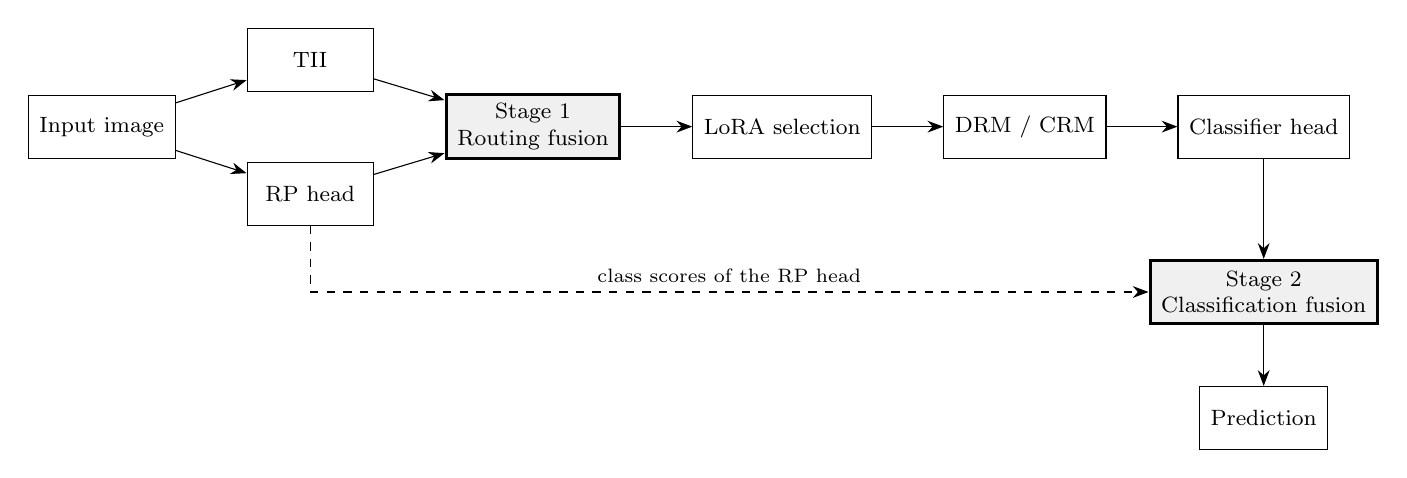
\begin{tikzpicture}[
  font=\footnotesize,
  >={Stealth[length=2mm]},
  box/.style={draw, minimum height=8mm, minimum width=1.6cm, inner xsep=4pt, align=center},
  hl/.style={box, very thick, fill=black!6}
]
% Each box is chained off the previous one's east edge, so what is specified is
% the GAP and the width is free to be whatever the label needs. Fixed centre
% coordinates cannot work here: box width depends on label length, so longer
% words silently eat the gap. With the old centres the LoRA-to-DRM gap fell to
% 1.49pt against a 2mm (5.69pt) arrow tip, i.e. the arrowhead was drawn inside
% the neighbouring box. 9mm keeps every gap at 25.61pt in both languages.
\node[box] (in) at (0, 0) {Input image};
\coordinate (up) at (0, 0.85);
\coordinate (dn) at (0,-0.85);
\coordinate (r1) at ([xshift=9mm]in.east);
\node[box, anchor=west] (tii) at (r1 |- up) {TII};
\node[box, anchor=west] (rp)  at (r1 |- dn) {RP head};
% anchored on rp, not tii: rp carries the longer label of the two, so it is the
% binding constraint if either label is ever edited.
\coordinate (r2) at ([xshift=9mm]rp.east);
\node[hl,  anchor=west] (f1) at (r2 |- in) {Stage 1\\Routing fusion};
\node[box, anchor=west] (lo) at ([xshift=9mm]f1.east) {LoRA selection};
\node[box, anchor=west] (dr) at ([xshift=9mm]lo.east) {DRM / CRM};
\node[box, anchor=west] (cl) at ([xshift=9mm]dr.east) {Classifier head};
\node[hl]  (f2) at ([yshift=-2.1cm]cl.center) {Stage 2\\Classification fusion};
\node[box] (out) at ([yshift=-3.7cm]cl.center) {Prediction};
\draw[->] (in) -- (tii);
\draw[->] (in) -- (rp);
\draw[->] (tii) -- (f1);
\draw[->] (rp) -- (f1);
\draw[->] (f1) -- (lo);
\draw[->] (lo) -- (dr);
\draw[->] (dr) -- (cl);
\draw[->] (cl) -- (f2);
\draw[->] (f2) -- (out);
\draw[->, dashed] (rp.south) |- node[pos=0.75, above, font=\scriptsize]
      {class scores of the RP head} (f2.west);
\end{tikzpicture}}
\caption{The inference pipeline. The bold-outlined blocks are the two added
components. The random-projection head is computed exactly once and feeds both
stages: task scores for the first, class scores for the second (dashed line).}
\label{fig:pipeline}
\end{figure}

\subsection{The Second Source of Evidence}

The second source must satisfy two constraints: it must add no trainable
parameters, since parameters updated by gradients across a task sequence can be
overwritten by later tasks; and it must preserve the exemplar-free protocol. A
second-order classification head in the style of RanPAC~\cite{ref_ranpac}
satisfies both.

The input feature $f \in \mathbb{R}^{d}$ with $d = 768$ is taken from the final
feature layer of ViT-B/16 after attaching \emph{one} fixed LoRA parameter set,
which serves as first-session adaptation. The index of that parameter set must be
fixed across all tasks; otherwise the accumulated terms below would mix
incompatible feature spaces.

\subsubsection{Projection and second-order statistics.}
The feature is projected into a high-dimensional space of size $M = 10^4$ and
passed through a nonlinearity, and the projected features are accumulated into
two matrices:
\begin{align}
h &= \mathrm{ReLU}(f W) \in \mathbb{R}^{M},
\qquad W \in \mathbb{R}^{d \times M} \text{ frozen, drawn from a fixed seed},
\label{eq:proj}\\
G &= \sum_n h_n h_n^{\top} \in \mathbb{R}^{M \times M},
\qquad
C = \sum_n h_n\, \mathbf{e}_{y_n}^{\top}
   \in \mathbb{R}^{M \times |\mathcal{Y}|},
\label{eq:gram}
\end{align}
where $\mathbf{e}_{y}$ is the basis vector of class $y$. The sums run over every
sample seen since the start of the sequence.

Going up in dimension is deliberate: in the original $768$-dimensional space the
classes overlap to the point that no hyperplane separates them, whereas after
the expansion a linear classifier becomes expressive enough. The nonlinearity is
mandatory rather than optional --- without it $fW$ is merely a linear transform
of $f$, of rank at most $d$, and projecting into $M \gg d$ dimensions adds no
separating power whatsoever.

\subsubsection{Classification by ridge regression.}
The output weights are the closed-form solution of a regularised least-squares
problem:
\begin{equation}
W_{\mathrm{out}} = (G + \lambda I)^{-1} C \in \mathbb{R}^{M \times |\mathcal{Y}|},
\qquad
s = h^{\top} W_{\mathrm{out}} \in \mathbb{R}^{|\mathcal{Y}|} .
\label{eq:ridge}
\end{equation}
There is no separate dimensionality-reduction step: $W_{\mathrm{out}}$ performs
it, collapsing $M$ dimensions down to $|\mathcal{Y}|$ in a single matrix
product. The trajectory of dimensions is
\begin{center}
$\underbrace{768}_{f}
\;\xrightarrow{\;\text{projection} + \text{nonlinearity}\;}\;
\underbrace{10^4}_{h}
\;\xrightarrow{\;W_{\mathrm{out}}\;}\;
\underbrace{|\mathcal{Y}|}_{s}$
\end{center}
We go up \emph{in order to make} the linear step down work. The Gram inverse is
the component that makes it work: the post-nonlinearity dimensions are strongly
correlated, and $(G + \lambda I)^{-1}$ decorrelates them.

\subsubsection{Two inherited properties.}
Both $G$ and $C$ in (\ref{eq:gram}) are \emph{sums} over samples, and addition
commutes, so for a \emph{fixed} feature map the accumulated statistics, and with
them $W_{\mathrm{out}}$, do not depend on the order in which the samples
arrived. Nothing an earlier task contributed is overwritten or decayed: the head
after $T$ tasks is the ridge solution of a joint fit over every feature seen so
far, and it reaches that solution having visited each task once.

This is weaker than an absence of forgetting and we claim no more than it says.
Adding a task adds classes that compete for the same arg max, so accuracy on old
classes can fall while their statistics sit untouched. Nor is the feature map
fixed across orderings: features come from the first task's adapter, so a
different task order yields a different extractor and a different $G$. The
property rules out one mechanism of forgetting --- the overwriting of old
evidence --- not the phenomenon. At the same time
the sizes of the two matrices do not depend on how many samples have been seen,
and no per-sample feature is ever retained, so the exemplar-free protocol is
preserved by the structure of the computation itself.

\subsection{Two-Stage Fusion}

Both stages blend two vectors that live on different scales: the ridge scores $s$
span roughly one unit while the logits $\ell$ span roughly thirty-five, so a
direct blend would let $\ell$ dominate at every weight. Each source is therefore
standardised per sample before blending:
\begin{equation}
z(v) = \frac{v - \mathrm{mean}(v)}{\mathrm{std}(v)} ,
\label{eq:znorm}
\end{equation}
with the mean and standard deviation computed separately for each sample, over
the classes seen so far only.

\subsubsection{First stage: fusion at the routing level.}
This stage runs \emph{before} any adapter is attached, so the routed logits
$\ell$ of (\ref{eq:logits}) do not exist yet; the signal it replaces is the
first matching step, and the scores it consumes are TII's own. Write
$u \in \mathbb{R}^{|\mathcal{Y}|}$ for the class scores of the auxiliary
classifier in (\ref{eq:tii}), taken before normalisation. Both $u$ and the
projection head's $s$ score \emph{classes}, whereas routing needs scores over
\emph{tasks}. We convert by taking the maximum over each task's class set, since
a task deserves to be selected when \emph{some} class of its own scores highly,
not when its classes score highly on average:
\begin{equation}
u^{\mathrm{task}}_t = \max_{c \in \mathcal{C}_t} u_c ,
\qquad
s^{\mathrm{task}}_t = \max_{c \in \mathcal{C}_t} s_c ,
\qquad t = 1,\dots,\hat{T},
\label{eq:taskscore}
\end{equation}
with $\hat{T}$ the number of tasks seen so far; classes of unseen tasks never
enter either maximum. The two vectors are blended after standardisation:
\begin{equation}
\mathrm{fused} = w\, z(u^{\mathrm{task}}) + (1-w)\, z(s^{\mathrm{task}}),
\qquad
\hat{t}_f = \arg\max_t\, \mathrm{fused}_t ,
\qquad w = 0.7 .
\label{eq:route}
\end{equation}
Two details of $z(\cdot)$ matter for reproduction. It divides by the
\emph{population} standard deviation, not the Bessel-corrected one, and floors
the divisor at $10^{-6}$. At the first stage $\hat{T}=1$, so the corrected
estimator divides by $\hat{T}-1=0$ and returns NaN, which no floor repairs;
the population estimator returns $0$ there, which the floor does repair. For
every later stage the two differ by a constant factor $\sqrt{\hat{T}/(\hat{T}-1)}$
shared by both sources, so it cancels in the arg max and moves no reported
number.
The identity $\hat{t}_f$ replaces the output of (\ref{eq:tii}) and is handed to
DRM and CRM as a better starting point. We replace \emph{exactly one} module, the
first matching step; every downstream mechanism is left untouched. At $w = 1.0$,
(\ref{eq:route}) returns exactly the ordering of $u^{\mathrm{task}}$, so
\emph{this stage} reduces to the baseline's first matching step. It does not by
itself recover the baseline: the second stage is governed by its own weight
$\beta$, and both $w=1.0$ and $\beta=0$ are needed for that.

\subsubsection{Second stage: gated fusion at the classification level.}
Because $\ell$ comes from the shared head, it frequently predicts the correct
class in spite of a wrong routing decision. We therefore use the
random-projection head itself as a secondary classifier, this time taking its
class scores $s$.

A fixed weight is the wrong instrument. It spends the same share of the decision
on a sample the primary head has already named with certainty as on one it is
hesitating over, and the former outnumber the latter overwhelmingly; paying there
only flattens a peak that was already correct. Fusion can change a prediction
only by unseating the top-ranked class, and its most plausible challenger is the
runner-up, so the weight is set in inverse proportion to the margin between the
two highest-scoring classes:
\begin{equation}
\beta_i = \beta \left( 1 - \frac{p_{(1)} - p_{(2)}}{p_{(1)} + p_{(2)}} \right),
\qquad \beta = 0.5 ,
\label{eq:gate}
\end{equation}
where $p_{(1)} \geq p_{(2)}$ are the two largest probabilities of
$\mathrm{softmax}(\ell)$ over the classes seen so far. Dividing by the sum makes
the quantity depend only on the ratio $p_{(2)}/p_{(1)}$, that is, it measures how
threatened the top class is, independently of how much probability mass the pair
holds. The gate closes on decided samples and opens on contested ones.

The blend reuses (\ref{eq:znorm}) and then maps the result back onto the scale of
$\ell$:
\begin{align}
m_i &= (1 - \beta_i)\, z(\ell_i) + \beta_i\, z(s_i),
\label{eq:mix}\\
\hat{\ell}_i &= m_i \cdot \mathrm{std}(\ell_i) + \mathrm{mean}(\ell_i)
   \in \mathbb{R}^{|\mathcal{Y}|}.
\label{eq:affine}
\end{align}
The map-back in (\ref{eq:affine}) is a per-sample affine transform with a
positive coefficient, so the ranking is unchanged; it is needed only for the
loss, because the mixture no longer sits on the scale of $\ell$, which is the
wrong scale for cross-entropy. It does not sit on unit scale either. For two
standardised vectors,
\begin{equation}
\mathrm{Var}\big((1-\beta) z_1 + \beta z_2\big)
  = (1-\beta)^2 + \beta^2 + 2\beta(1-\beta)\rho ,
\label{eq:mixvar}
\end{equation}
with $\rho$ their correlation across classes; this equals one only when
$\rho = 1$, and at $\beta = 0.5$ with uncorrelated sources it is $0.5$. The
map-back therefore returns the scores to a reference scale. It is not a variance
guarantee and not a calibration argument, and we make no calibration claim: the
loss we report is cross-entropy at that scale, not a measure of reliability. At
$\beta = 0$ we have $\hat{\ell} = \ell$ element-wise, so this stage also reduces
exactly to the baseline.

\subsubsection{Cost.}
At inference the head costs one extra adapter forward per sample, and the same
result serves both stages. That is the head's own cost, not the pipeline's
difference: changing the initial route also changes how many candidates DRM and
CRM go on to examine, and we did not measure that second-order effect.

Per task the head accumulates $G$ and $C$ over the current task's training split
and solves one ridge system, so its footprint is set by $M$ and not by how many
samples have been seen. That footprint is not small. At $M = 10^4$ the Gram
matrix holds $10^8$ entries, $800$~MB in the float64 the solve requires; the
Cholesky factor and the regularised copy it consumes bring the peak near
$2.4$~GB. A complete ten-task evaluation on ImageNet-R --- statistics, ten
solves and all inference --- takes $283$~s on one RTX 4090 at batch $24$. We
report the total because we did not instrument the three phases separately.

\section{Experimental Setup}
\label{sec:setup}

The backbone is a ViT-B/16 pre-trained on ImageNet-21K and adapted with LoRA of
rank $8$. The four-seed study of Sect.~\ref{sec:results} uses Split-ImageNet-R,
Split-CIFAR100 and Split-CUB200, each divided into $10$ tasks; the grid of
Sect.~\ref{sec:grid} replaces CUB-200 with Split-ImageNet-A and 5-Datasets, the
latter being a $5$-task sequence. Every experiment is repeated over four seeds,
$42$ through $45$; the LoRA pool and the TII module are retrained from scratch
for each seed. Baseline and proposed
method are evaluated from the same checkpoints through the same code path, so a
reported difference reflects the inference-time change alone and carries no
training noise. The random-projection head uses $M = 10^4$ dimensions, a ReLU
non-linearity and ridge parameter $\lambda = 10^4$; no temperature scaling is
applied.

Writing $a_{i,t}$ for the accuracy on task $i$ measured at stage $t$, we report
routing accuracy (Acc@task), classification accuracy at ranks one and five
(Acc@1, Acc@5), cross-entropy Loss, and the two retention measures
\begin{equation}
\mathrm{Forgetting} = \frac{1}{T-1}\sum_{i=1}^{T-1}
\Big( \max_{1 \le t \le T} a_{i,t} - a_{i,T} \Big),
\qquad
\mathrm{Backward} = \frac{1}{T-1}\sum_{i=1}^{T-1} \big( a_{i,T} - a_{i,i} \big).
\label{eq:metrics}
\end{equation}
Both averages run over the $T-1$ tasks that precede the last one. The final
task is excluded because it contributes an identically zero term to each sum:
it has been evaluated at one stage only, so its maximum and its final accuracy
are the same entry. Including it would divide a fixed numerator by $T$ instead
of $T-1$ and report every retention figure a factor $(T-1)/T$ too small --- on
our ten-task benchmarks, $10\%$ low. The maximum runs over the stages at which
task $i$ was actually evaluated, that is $t \ge i$; the unevaluated lower
triangle of the accuracy matrix never enters either statistic.

Lower is better for Loss and Forgetting, higher for the rest. Both retention
measures compare a task against \emph{itself} at an earlier stage rather than
against another method, which is what makes them behave differently from the
accuracy axes in Sect.~\ref{sec:results}.

\subsubsection{Sanity check on the implementation.}
Setting $w = 1.0$ in (\ref{eq:route}) puts the whole routing weight on TII, and
setting $\beta = 0$ in (\ref{eq:mix}) leaves $\hat{\ell} = \ell$ element-wise.
Both are required: each governs one stage, and $w = 1.0$ alone still leaves the
classification stage blending. With the pair set, the projection head is off at
every point it acts, and the method reproduces the HRM-PET baseline digit for
digit on all three datasets --- $77.7914$, $74.0191$, $1.2305$ and the remainder
agree to the fourth decimal. Every difference in Table~\ref{tab:main} therefore
comes from the added components rather than from an incidental difference in the
evaluation path, and $w$ and $\beta$ each double as a continuous ablation axis
for the stage it controls.

\section{Results}
\label{sec:results}

Table~\ref{tab:main} reports all three datasets. Values are the mean $\pm$
standard deviation over four seeds. The change column is computed pairwise ---
the difference between proposed and baseline is taken per seed and only then
averaged --- so its standard deviation describes the stability of the
improvement itself rather than the varying difficulty of the seeds.

\begin{table}
\small
\setlength{\tabcolsep}{4.5pt}
\caption{Results on three datasets, mean $\pm$ standard deviation over seeds
42--45.}\label{tab:main}
\begin{tabular}{llrrr}
\hline
\multicolumn{2}{l}{Dataset and metric} & HRM-PET & Proposed & Change\\
\hline
\multicolumn{5}{l}{\emph{Split-ImageNet-R}}\\
& Acc@task   & $77.58 \pm 0.33$ & $79.85 \pm 0.18$ & $+2.264 \pm 0.158$\\
& Acc@1      & $73.94 \pm 0.48$ & $75.18 \pm 0.24$ & $+1.236 \pm 0.416$\\
& Acc@5      & $86.71 \pm 0.21$ & $88.02 \pm 0.17$ & $+1.312 \pm 0.148$\\
& Loss       & $1.23 \pm 0.01$  & $1.19 \pm 0.01$  & $-0.040 \pm 0.002$\\
& Forgetting & $3.36 \pm 0.56$  & $3.30 \pm 0.35$  & $-0.056 \pm 0.334$\\
& Backward   & $-3.16 \pm 0.61$ & $-3.20 \pm 0.42$ & $-0.047 \pm 0.282$\\
\multicolumn{5}{l}{\emph{Split-CIFAR100}}\\
& Acc@task   & $89.77 \pm 0.11$ & $90.87 \pm 0.09$ & $+1.103 \pm 0.066$\\
& Acc@1      & $89.78 \pm 0.03$ & $90.47 \pm 0.05$ & $+0.690 \pm 0.063$\\
& Acc@5      & $98.65 \pm 0.03$ & $98.86 \pm 0.07$ & $+0.217 \pm 0.057$\\
& Loss       & $0.39 \pm 0.00$  & $0.39 \pm 0.00$  & $-0.000 \pm 0.001$\\
& Forgetting & $3.89 \pm 0.08$  & $3.74 \pm 0.12$  & $-0.156 \pm 0.098$\\
& Backward   & $-3.87 \pm 0.07$ & $-3.73 \pm 0.11$ & $+0.142 \pm 0.097$\\
\multicolumn{5}{l}{\emph{Split-CUB200}}\\
& Acc@task   & $93.12 \pm 0.14$ & $94.34 \pm 0.10$ & $+1.226 \pm 0.149$\\
& Acc@1      & $86.38 \pm 0.25$ & $87.88 \pm 0.27$ & $+1.495 \pm 0.353$\\
& Acc@5      & $97.04 \pm 0.10$ & $97.44 \pm 0.13$ & $+0.400 \pm 0.103$\\
& Loss       & $0.57 \pm 0.00$  & $0.53 \pm 0.01$  & $-0.036 \pm 0.004$\\
& Forgetting & $2.54 \pm 0.35$  & $2.18 \pm 0.12$  & $-0.359 \pm 0.325$\\
& Backward   & $-2.42 \pm 0.39$ & $-2.14 \pm 0.13$ & $+0.279 \pm 0.391$\\
\hline
\end{tabular}
\end{table}

The six metrics are not six independent events; they measure three axes, and
reporting by axis says more than a pooled count. The deciding quantity is the
ratio of a change to the standard deviation of that same change: below $2$ it is
not resolved.

\subsubsection{Routing (Acc@task): improved.}
The gain is $+1.10$ to $+2.26$ points at ratios between $8$ and $17$. This is
the axis the first stage acts on directly and it carries the firmest evidence.

\subsubsection{Classification (Acc@1, Acc@5): improved.}
Acc@1 rises by $+0.69$ to $+1.50$ points at ratios of $3.0$ to $11.0$, Acc@5 by
$+0.22$ to $+1.31$ at $3.8$ to $8.9$. Routing gains do not convert fully into
classification gains --- Sect.~\ref{sec:method} explains why the shared head
often predicts the right class in spite of a wrong route --- but the part that
does convert repeats across every seed.

\subsubsection{Retention (Forgetting, Backward): small, and mostly unresolved.}
Read as paired differences over the four seeds, the $95\%$ interval from $t_3$
covers zero in five of the six retention cells. The exception is Forgetting on
CIFAR-100, $-0.156$ with interval $[-0.312, -0.000]$, which sits on the
boundary. The two metrics are near mirror images --- $-0.156$ against $+0.142$
on CIFAR-100, $-0.359$ against $+0.279$ on CUB-200 --- so counting them as two
results counts one event twice. We therefore claim no consistent improvement on
this axis. That is not a claim of equivalence: with four seeds the intervals
are wide enough to hold differences that would matter, and we did not fix a
margin in advance against which to test one. What \emph{is} resolved is the
decomposition of Sect.~\ref{sec:grid} --- the accuracy retained on earlier tasks
rises in every grid cell, and Backward stays near zero only because the accuracy
at learning time rises with it.

\subsection{The Full Grid}
\label{sec:grid}

Everything above rests on one backbone. The original work states experiments on
four datasets under five pre-training configurations. Its own ablation table
names the five --- Sup-21K, iBOT-21K, iBOT-1K, DINO-1K and MoCo-1K --- and three
traces in its released code identify the four datasets and corroborate that
list: four pairs of configuration files (CIFAR-100, ImageNet-R, ImageNet-A,
5-Datasets, and no CUB-200) and a stray \texttt{.DS\_Store} in
\texttt{training\_scripts/} listing twenty script names, i.e.\ four datasets
times five backbones. We rebuilt all twenty cells, retraining the entire HRM-PET
pipeline from scratch wherever checkpoints were missing, and evaluated baseline
and proposed method through one code path at one seed.

\begin{table}
\small
\setlength{\tabcolsep}{4.5pt}
\caption{The full grid: four datasets by the five pre-training configurations of
the original work. Acc@1 at seed 42; HRM-PET is $w=1$, $\beta=0$ and Proposed is
$w=0.7$, $\beta=0.5$. 5-Datasets is a sequence of five datasets and therefore has
five tasks by definition; the other three split their classes into ten.
$\Delta$ is the proposed method minus the HRM-PET row.}
\label{tab:grid}
\begin{tabular}{llrrrrr}
\hline
Dataset & & Sup-21K & MoCo-1K & iBOT-1K & iBOT-21K & DINO-1K\\
\hline
ImageNet-R & HRM-PET  & 74.02 & 68.47 & 71.89 & 73.29 & 70.23\\
           & $\Delta$ & $+1.49$ & $+1.89$ & $+2.52$ & $+2.55$ & $+2.68$\\
CIFAR-100  & HRM-PET  & 89.77 & 85.50 & 86.46 & 88.52 & 85.36\\
           & $\Delta$ & $+0.76$ & $+2.12$ & $+2.06$ & $+1.80$ & $+2.03$\\
ImageNet-A & HRM-PET  & 45.85 & 31.80 & 37.08 & 41.48 & 36.44\\
           & $\Delta$ & $+1.57$ & $+2.41$ & $+3.58$ & $+2.63$ & $+0.97$\\
5-Datasets & HRM-PET  & 91.37 & 92.63 & 93.80 & 93.83 & 92.52\\
           & $\Delta$ & $+2.40$ & $+1.41$ & $+0.85$ & $+0.59$ & $+0.75$\\
\hline
\end{tabular}
\end{table}

Table~\ref{tab:grid} reports all of them. \emph{Every cell} improves on both
accuracy axes --- Acc@task by $+0.97$ to $+4.57$, Acc@1 by $+0.59$ to $+3.58$
--- while the baselines span nearly a factor of three, from $31.8$ to $93.8$.

Absolute differences are hard to compare across cells starting $50$ points
apart. In relative error reduction 5-Datasets has the smallest absolute gains
--- as little as $+0.59$ --- and the largest relative ones, $9.6\%$ to
$27.8\%$, its baselines being already at $91$--$94$; ImageNet-A is the converse,
where $+2.41$ and $+2.63$ amount to $3.5\%$ and $4.5\%$ against baselines in the
thirties and forties.

Retention over the same twenty cells behaves in a way the summary metrics hide.
Writing $a_{i,T}$ for the final accuracy on task $i$ and $a_{i,i}$ for the
accuracy it reached when it was learned, Backward averages their difference, so
it charges a method for learning better. Both halves rise here: against the
baseline the final accuracy on earlier tasks improves in \emph{every one} of the
twenty cells, by $+1.83$ on average, and the accuracy at learning time improves
by $+1.58$. Backward is the small residue of two larger movements, and it
worsens in five of the twenty cells --- every one of them a cell where the gain
at learning time exceeded the gain retained, not a cell that forgot more.

\section{Ablation}
\label{sec:ablation}

The original work ablates \emph{cumulatively}: each row adds exactly one
component to the row above, measured on ImageNet-R with the pre-training
configurations as columns. Table~\ref{tab:cumul} rebuilds that shape for our two
stages, so the two ablations can be read side by side.

\begin{table}
\small
\setlength{\tabcolsep}{4.5pt}
\caption{Ablation on Split-ImageNet-R, seed 42, Acc@1, in the cumulative shape
the original work uses. Two pairs of rows differ in the routing stage alone
--- with the gate off (rows three and four) and with it on (rows five and six)
--- which is what exposes the interaction between the two stages. Unlike the
corresponding table of the original work this one is a single seed and carries
no standard deviation; Table~\ref{tab:classonly} repeats the decisive comparison
over four seeds.}
\label{tab:cumul}
\begin{tabular}{lrrrrr}
\hline
& Sup-21K & MoCo-1K & iBOT-1K & iBOT-21K & DINO-1K\\
\hline
Baseline ($w=1$, $\beta=0$)             & 74.02 & 68.47 & 71.89 & 73.29 & 70.23\\
Baseline $+$ routing ($w=0.7$)          & 74.31 & 68.81 & 72.46 & 73.91 & 70.97\\
Baseline $+$ class ($\beta=0.5$)        & 74.53 & 70.70 & 74.96 & 75.72 & 72.91\\
Baseline $+$ routing $+$ class          & 74.55 & 70.63 & 74.95 & 75.72 & 72.87\\
Baseline $+$ class $+$ gate             & 75.38 & 70.08 & 73.64 & 75.41 & 72.14\\
Baseline $+$ routing $+$ class $+$ gate & 75.51 & 70.37 & 74.41 & 75.84 & 72.91\\
\hline
\multicolumn{6}{l}{\emph{Isolated contribution over the baseline}}\\
routing alone & $+0.29$ & $+0.34$ & $+0.57$ & $+0.62$ & $+0.74$\\
class alone   & $+0.51$ & $+2.23$ & $+3.07$ & $+2.43$ & $+2.68$\\
\multicolumn{6}{l}{\emph{Marginal contribution of routing}}\\
given class            & $+0.02$ & $-0.07$ & $-0.01$ & $\ \ 0.00$ & $-0.04$\\
given class and gate   & $+0.13$ & $+0.29$ & $+0.77$ & $+0.43$ & $+0.77$\\
\multicolumn{6}{l}{\emph{Marginal contribution of the gate}}\\
given class            & $+0.85$ & $-0.62$ & $-1.32$ & $-0.31$ & $-0.77$\\
given routing and class & $+0.96$ & $-0.26$ & $-0.54$ & $+0.12$ & $+0.04$\\
\hline
\end{tabular}
\end{table}

\subsubsection{On Acc@1 the two stages overlap, and the gate decides how much.}
Each stage alone beats the baseline on every backbone --- routing by $+0.29$ to
$+0.74$, the classifier by $+0.51$ to $+3.07$ --- and they are far from additive.
With the gate off they are almost entirely redundant: adding routing to the
classifier moves Acc@1 by $-0.07$ to $+0.02$, so whatever the routing stage
repairs, the classification stage was going to repair anyway. This is the second
weakness of Sect.~\ref{sec:related} measured as an interaction rather than
asserted: because the shared head spans every seen class, a corrected route
mostly changes which adapter produced a prediction that was already right.

The redundancy is conditional, and reporting only the ungated pair would have
made it look absolute. With the gate on, routing is worth $+0.13$ to $+0.77$ and
is positive on all five backbones. The dependence runs the other way too: the
gate costs $-1.32$ to $+0.85$ when the classifier is alone and only
$-0.54$ to $+0.96$ once routing is present. Each repairs what the other breaks.
The gate withholds the projection head exactly where the routed head is
confident, and a wrong route is one of the things that makes it confident for
the wrong reason; correcting the route first is what makes that withholding
safe.

A single seed cannot settle a difference of a few tenths, so
Table~\ref{tab:classonly} repeats the comparison that matters --- the full
method against its second stage alone --- over four seeds on the three
benchmarks of Sect.~\ref{sec:results}.

\begin{table}
\small
\setlength{\tabcolsep}{4.5pt}
\caption{The second stage alone against the full method, Acc@1, mean $\pm$
standard deviation over seeds 42--45. The last two rows give the paired
difference and its $95\%$ confidence interval, from $t_3$ on the four per-seed
differences.}
\label{tab:classonly}
\begin{tabular}{lrrr}
\hline
& Split-ImageNet-R & Split-CIFAR100 & Split-CUB200\\
\hline
HRM-PET                       & $73.94 \pm 0.48$ & $89.78 \pm 0.03$ & $86.38 \pm 0.25$\\
Class stage only              & $74.49 \pm 0.14$ & $90.15 \pm 0.16$ & $88.01 \pm 0.21$\\
Both stages, gated (proposed) & $75.18 \pm 0.24$ & $90.47 \pm 0.05$ & $87.88 \pm 0.27$\\
\hline
Paired difference & $+0.69$ & $+0.33$ & $-0.13$\\
$95\%$ CI & $[+0.36, +1.01]$ & $[+0.03, +0.62]$ & $[-0.48, +0.23]$\\
\hline
\end{tabular}
\end{table}

Over four seeds the first stage earns its place on two benchmarks of three: the
interval excludes zero on ImageNet-R and on CIFAR-100, and the difference is
positive on every individual seed of both. On CUB-200 it does not: the
difference is $-0.13$ with an interval spanning zero, so on that benchmark the
classification stage alone is as good as the full method and possibly better.
We state that rather than average it away. CIFAR-100 carries the most weight of
the three, because it is the one benchmark in this table on which no
hyper-parameter was chosen; had the effect appeared only on ImageNet-R, where
$w$, $\beta$ and the gate were all selected, it could not be separated from
selection bias.

The first stage is also the only component that moves Acc@task, by $+2.18$ to
$+3.95$ (Table~\ref{tab:grid}), an axis a routing method reports in its own
right. But a reader should not add the two Acc@1 contributions together, and an
earlier version of this ablation, which reported only the nested chain, invited
exactly that error. Note also that the classifier's isolated contribution is by
far the smallest on Sup-21K, $+0.51$ against $+2.23$ to $+3.07$ on the other
four --- and Sup-21K is the backbone every design decision in
Sect.~\ref{sec:results} was taken on.

\subsubsection{The gate helps where it was tuned and costs elsewhere.}
At the published $\beta$ the gate is worth $+0.96$ on Sup-21K, is neutral on
iBOT-21K and DINO, and removes $0.26$ to $0.54$ points on MoCo and iBOT-1K. That
comparison is not fair to the ungated arm: $\beta=0.5$ was chosen \emph{with} the
gate active, so it pits a tuned configuration against an untuned one. The fair
version gives the ungated arm its own best value, $\beta=0.3$ in our sweep of
$\beta \in \{0.3,0.5,0.8,1.0\}$, and runs both arms over the whole grid;
Table~\ref{tab:gate-cross} is that comparison.

\begin{table}
\small
\setlength{\tabcolsep}{4.5pt}
\caption{Acc@1 change from removing the gate and lowering $\beta$ to $0.3$,
against the published configuration (gate on, $\beta=0.5$). Positive means
\emph{removing the gate is better}. Seed 42.}
\label{tab:gate-cross}
\begin{tabular}{lrrrrrr}
\hline
& Sup-21K & MoCo-1K & iBOT-1K & iBOT-21K & DINO-1K & Mean\\
\hline
ImageNet-R & $-0.09$ & $+0.78$ & $+0.80$ & $+0.51$ & $+0.60$ & $+0.52$\\
CIFAR-100  & $0.00$  & $+0.57$ & $+0.80$ & $+0.56$ & $+0.83$ & $+0.55$\\
ImageNet-A & $+0.14$ & $-0.14$ & $+0.06$ & $+0.89$ & $+0.46$ & $+0.28$\\
5-Datasets & $-0.13$ & $-0.26$ & $-0.19$ & $-0.26$ & $-0.99$ & $-0.37$\\
\hline
\end{tabular}
\end{table}

\subsubsection{Across the grid the picture reverses by dataset.}
Table~\ref{tab:gate-cross} extends the comparison to all four benchmarks.
Removing the gate wins on ImageNet-R and CIFAR-100, roughly ties on ImageNet-A,
and \emph{loses on all five cells} of 5-Datasets; over the twenty grid cells it
is ahead by $0.25$ points. The shape matches what the gate is for. It mixes the
second stage only into samples the primary model is not already sure about, and
on 5-Datasets the baseline is at $91.4$--$93.8$ Acc@1, so nearly every sample is
both correct and confident --- exactly the samples the gate protects. On
ImageNet-R ($68$--$74$) and CIFAR-100 ($85$--$90$) enough samples remain wrong
that mixing unconditionally pays.

We keep the gate, and state the reasoning rather than the conclusion. It wins on
the benchmark furthest from the one it was tuned on, which is transfer evidence
rather than fitting evidence; it makes the method insensitive to $\beta$, which
matters because we do not tune $\beta$ per dataset; and what it costs is half a
point on two benchmarks against up to one point on the third. We record that we
nearly discarded it on ImageNet-R evidence alone, because that is precisely the
trap Sect.~\ref{sec:limits} warns about. One caveat completes the picture: the
ungated arm reaches higher Acc@1 on ImageNet-R and CIFAR-100 but its Loss on
CIFAR-100 is worse by $+0.019 \pm 0.003$ over three seeds. Mixing unconditionally
fixes more labels while making the probability distribution worse.

\section{Limitations}
\label{sec:limits}

Hyper-parameters were selected on ImageNet-R, so that dataset does not
contribute independent evidence; the $11$ cells of CIFAR-100 and CUB-200 do.
The four-seed protocol covers one backbone, and the $21$-cell grid covers one
seed; no cell has both. We claim nothing on the retention axis, where no change
reaches the resolution threshold. Finally, the method inherits whatever the
frozen pipeline provides: it never modifies training, so the error that remains
when routing is correct and both heads are consulted lies outside its reach.

\section{Conclusion}

Two fusion stages, both at inference and neither requiring retraining, improve
two of the three axes measured: routing by $+1.10$ to $+2.26$ points and
classification by $+0.69$ to $+1.50$ points, across three datasets and four
seeds, by several times the seed-to-seed standard deviation. The retention axis
shows no change distinguishable from zero and we claim none. The first stage
exploits the complementarity of two routing signals that fail on different
samples; the second exploits the fact that the second signal is already a
complete classifier that the original architecture discards.

What makes us believe the result is not a property of one backbone or one
dataset is the full grid: over the four datasets and five backbones the original
work covers, no cell moves the wrong way on
either accuracy axis, and it does so over baselines spanning nearly a factor of
three, from $31.8$ to $93.8$ Acc@1. Read as relative error reduction the effect
is largest where the baseline is strongest, up to $27.8\%$ on 5-Datasets, which
is where an absolute reading makes the method look weakest.

%
\begin{credits}
\subsubsection{\ackname}
We thank our supervisor for comments on this manuscript.

% The Disclosure of Interests block was removed on request. Springer requires
% it for an actual proceedings submission, so restore it before submitting:
%   \subsubsection{\discintname}
%   The authors declare that they have no competing interests related to the
%   content of this article.
\end{credits}
%
% ---- Bibliography ----
%
% NOTE: the entries below were transcribed from the reference list of the
% HRM-PET paper. Before the final submission each one must be checked against
% the original publication: years and author-name spellings may differ. If
% BibTeX is used, declare \bibliographystyle{splncs04}.
%
\begin{thebibliography}{8}

\bibitem{ref_hrmpet}
Wang, W., Jia, G., Liu, X., Lin, L., Yang, J.: Hybrid re-matching for continual
learning with parameter-efficient tuning. In: NeurIPS (2025)

\bibitem{ref_ranpac}
McDonnell, M.D., Gong, D., Parvaneh, A., Abbasnejad, E., van den Hengel, A.:
RanPAC: random projections and pre-trained models for continual learning. In:
NeurIPS (2023)

\bibitem{ref_hide}
Wang, L., Xie, J., Zhang, X., Huang, M., Su, H., Zhu, J.: Hierarchical
decomposition of prompt-based continual learning: rethinking obscured
sub-optimality. In: NeurIPS (2023)

\bibitem{ref_l2p}
Wang, Z., Zhang, Z., Lee, C.Y., Zhang, H., Sun, R., Ren, X., Su, G., Perot, V.,
Dy, J., Pfister, T.: Learning to prompt for continual learning. In: CVPR (2022)

\bibitem{ref_dualprompt}
Wang, Z., Zhang, Z., Ebrahimi, S., Sun, R., Zhang, H., Lee, C.Y., Ren, X., Su,
G., Perot, V., Dy, J., et al.: DualPrompt: complementary prompting for
rehearsal-free continual learning. In: ECCV (2022)

\bibitem{ref_lora}
Hu, E.J., Shen, Y., Wallis, P., Allen-Zhu, Z., Li, Y., Wang, S., Wang, L., Chen,
W.: LoRA: low-rank adaptation of large language models. In: ICLR (2022)

% The nine entries below were added with the Related Work section. Every author
% list has been checked against the paper itself; ref_adam had been missing
% Z.-W. Cai and ref_dlepem had no authors at all, and both are now complete.

\bibitem{ref_coda}
Smith, J.S., Karlinsky, L., Gutta, V., Cascante-Bonilla, P., Kim, D., Arbelle,
A., Panda, R., Feris, R., Kira, Z.: CODA-Prompt: continual decomposed
attention-based prompting for rehearsal-free continual learning. In: CVPR (2023)

\bibitem{ref_adam}
Zhou, D.W., Cai, Z.W., Ye, H.J., Zhan, D.C., Liu, Z.: Revisiting
class-incremental learning with pre-trained models: generalizability and
adaptivity are all you need. Int. J. Comput. Vis. (2024)

\bibitem{ref_survey}
Masana, M., Liu, X., Twardowski, B., Menta, M., Bagdanov, A.D., van de Weijer,
J.: Class-incremental learning: survey and performance evaluation on image
classification. IEEE Trans. Pattern Anal. Mach. Intell. (2023)

\bibitem{ref_icarl}
Rebuffi, S.A., Kolesnikov, A., Sperl, G., Lampert, C.H.: iCaRL: incremental
classifier and representation learning. In: CVPR (2017)

\bibitem{ref_bic}
Wu, Y., Chen, Y., Wang, L., Ye, Y., Liu, Z., Guo, Y., Fu, Y.: Large scale
incremental learning. In: CVPR (2019)

\bibitem{ref_wa}
Zhao, B., Xiao, X., Gan, G., Zhang, B., Xia, S.T.: Maintaining discrimination
and fairness in class incremental learning. In: CVPR (2020)

\bibitem{ref_lucir}
Hou, S., Pan, X., Loy, C.C., Wang, Z., Lin, D.: Learning a unified classifier
incrementally via rebalancing. In: CVPR (2019)

\bibitem{ref_mote}
Li, L., Wu, Z., Ji, Y.: MoTE: mixture of task-specific experts for pre-trained
model based class-incremental learning. Knowledge-Based Systems (2025)

\bibitem{ref_dlepem}
Zhao, H., Liu, R., Liu, Y.: Dynamic LoRA-experts and prototype-ensemble matching
for class-incremental learning. Applied Sciences \textbf{16}(12), 6153 (2026)

\end{thebibliography}
\end{document}
